\documentclass[]{article}
\usepackage[utf8]{inputenc}
\usepackage[T1]{fontenc}
\usepackage[spanish]{babel}
\usepackage{enumerate}
\usepackage[sorting=none]{biblatex}
\usepackage{float}
\usepackage{graphicx}

%--------DATE---------%
\usepackage[yyyymmdd]{datetime}
\renewcommand{\dateseparator}{--}

%--------BIBLIOGRAPHY---------%
\bibliography{treesBib.bib} 


\title{\textbf{Diferentes Árboles como estructuras de datos}}
\author{Daniel E. Hernández - \texttt{20180077}}

\begin{document}

\maketitle

\begin{abstract}
El siguiente documento busca explicar diferentes tipos de árboles utilizados como estructuras de datos. 
\end{abstract}

\section{Huffman Tree}
	\subsection{Definición:}
		\par En 1951, David A. Huffman y sus compañeros de clase de teoría de la información del MIT tuvieron la oportunidad de elegir entre un trabajo trimestral o un examen final. El profesor, Robert M. Fano, asignó un trabajo sobre el problema de encontrar el código binario más eficiente. Huffman, incapaz de probar que ninguno de los códigos era el más eficiente, estaba a punto de abandonar y comenzar a estudiar para el final cuando se le ocurrió la idea de usar un árbol binario clasificado por frecuencias y rápidamente demostró que este método era el más eficiente.
		
		\par Al hacerlo, Huffman superó a Fano, quien había trabajado con el inventor de la teoría de la información Claude Shannon para desarrollar un código similar. Construir el árbol de abajo hacia arriba garantiza la optimización, a diferencia de la codificación Shannon-Fano de arriba hacia abajo.\cite{stixScientificAmericanArticle1991}
	\subsection{Casos de uso:}
		\begin{enumerate}
			\item \textbf{FLAC}: Compresión \textit{lossless} de audio.\cite{instituteofelectricalandelectronicsengineers20164thInternational2016}
			\item \textbf{GZIP}: Compresión \textit{lossless} de archivos. \cite{freesoftwarefundationGNUGzip2008}
			\item \textbf{PNG}: Compresión \textit{lossless} de imágenes. \cite{libpngPNGSpecificationDeflate}
			\item \textbf{MP3}: \textit{Encoding} de archivos de audio con compresión \textit{lossy} (no utiliza el algoritmo para comprimir, lo utiliza únicamente para \textit{encoding}). \cite{MP3TechOverview}
		\end{enumerate}
	\subsection{Implementación:}
		\begin{enumerate}
			\item Cree un nodo hoja para cada símbolo y añadirlo a la cola de prioridades.
			\item Mientras haya más de un nodo en la cola:
			\item Eliminar los dos nodos de mayor prioridad (menor frecuencia) de la cola
			\item Cree un nuevo nodo interno con estos dos nodos hijos y con un valor frecuencia igual a la suma de las frecuencias de los dos nodos.
			\item Añada el nuevo nodo a la cola.
			\item El nodo restante es el nodo raíz y el árbol está completo.
		\end{enumerate}
	\subsection{Ejemplo en graphviz:}
	\begin{figure}[H]
		\centering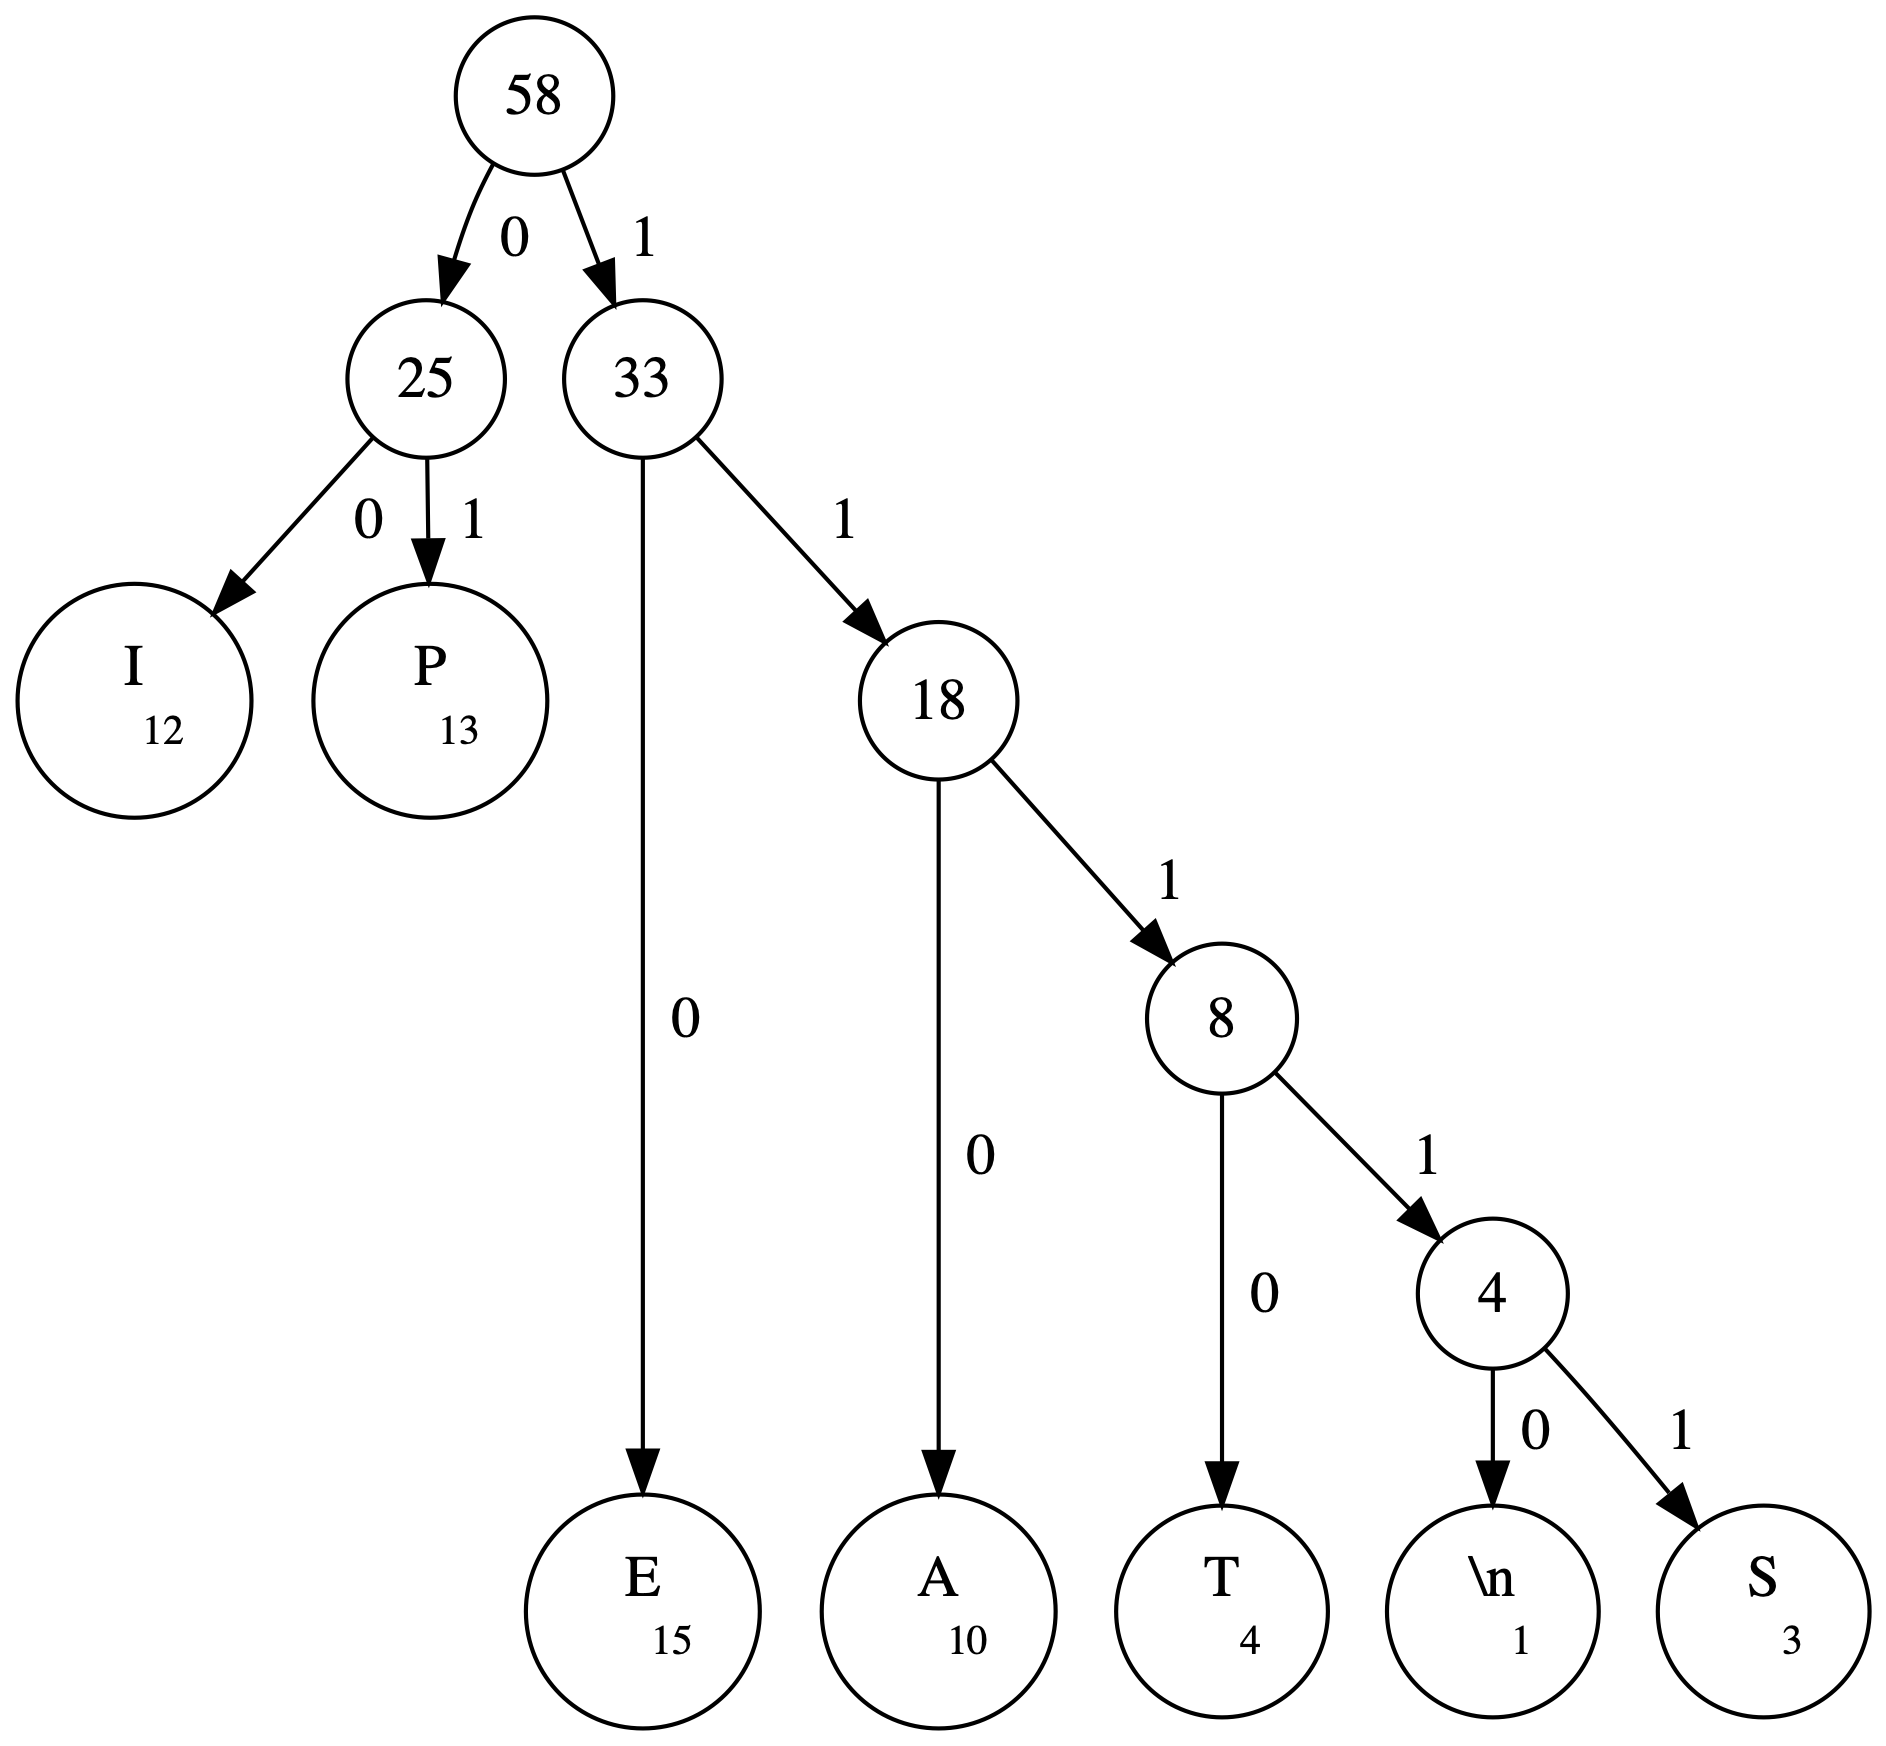
\includegraphics[width=\textwidth]{graphviz/huffman.png}
		\caption{Huffman Aplicado}
		\label{fig:Huffman Aplicado}
	\end{figure}


\section{Min Binary Heap Tree}
	\subsection{Definición:}
		\par El \textit{Binary Heap Tree} fue introducido en 1964 por J. W. J. Williams como una estructura de datos para hacer \emph{sorting.}\cite{forsytheAlgorithms1964} Este es un árbol de tipo completo y en el caso de ser un min-heap, el nodo padre es por definición siempre menor que su(s) respectivos nodos hijos. 
	\subsection{Casos de uso:}
		\begin{enumerate}
			\item \textbf{Ordenamiento estadístico}: Ordenar un arreglo de datos de menor a mayor en $O(\log_{}n)$.
			\item \textbf{Colas de prioridad}: Un ejemplo podría ser cambiarle de prioridad a un cliente dependiendo qué tanto se tarde el restaurante en servirle a él.
			\item \textbf{Planificadores}: Un organizador de tareas en base a una prioridad dada por el usuario.
		\end{enumerate}
	\subsection{Implementación:}
		\subsubsection{Insertar:}
			\begin{enumerate}
				\item Se inserta un elemento en el próximo espacio disponible (abajo-derecha).
				\item Se compara su valor con el nodo padre.
				\item Mientras el valor del nodo insertado sea mayor que el del nodo padre, se intercambian de lugar ambos nodos.
			\end{enumerate}
		\subsubsection{Remover:}
			\begin{enumerate}
				\item Se remueve el nodo raíz.
				\item Se copia el último nodo insertado en la posición raíz.
				\item Mientras el valor del nuevo nodo raíz sea mayor que el de alguno de sus hijos, se intercambia con el menor de ellos.
			\end{enumerate}
	\subsection{Ejemplo en graphviz:}
		\begin{figure}[H]
			\centering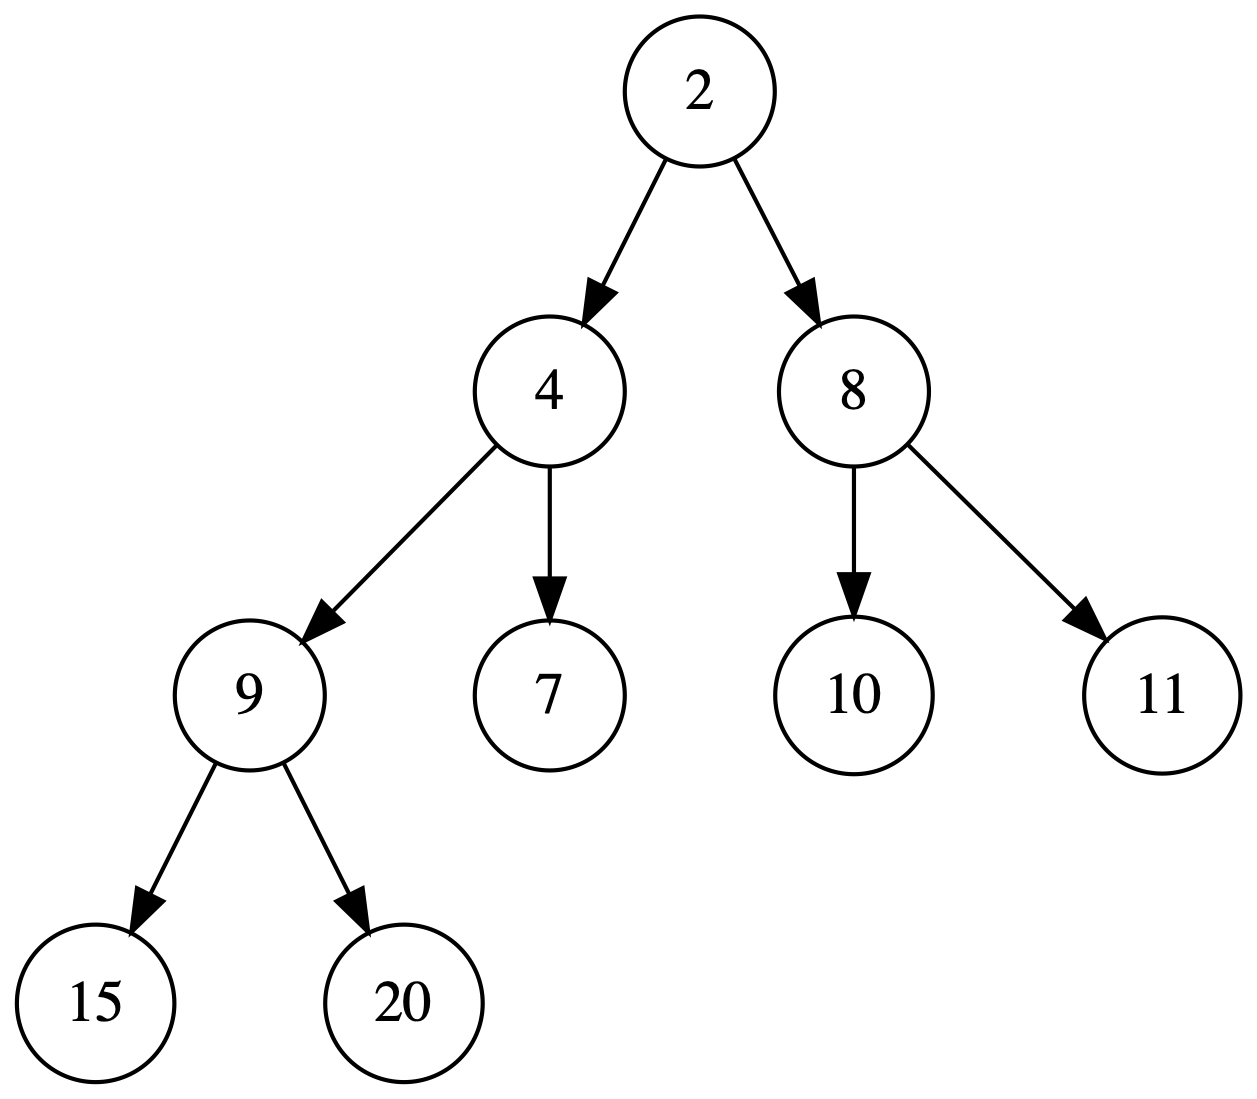
\includegraphics[width=\textwidth]{graphviz/minBinaryHeapTree.png}
			\caption{Min Binary Heap Tree}
			\label{fig:Min Binary Heap Tree}
		\end{figure}
	

\section{Treap}
	\subsection{Definición:}
		\par El \textit{Treap} fue descrito por primera vez por Raimund Seidel y Cecilia R. Aragón en 1989\cite{symposiumonfoundationsofcomputerscience30thAnnualSymposium1989}; su nombre es un \textit{portmanteau} de árbol \textit{(tree)} y pila \textit{(heap)}. Es un árbol cartesiano en el que cada nodo tiene una prioridad numérica (elegida al azar). 
		
		\par Al igual que con cualquier árbol de búsqueda binario, el orden de paso de los nodos es el mismo que el orden  de las claves. La estructura del árbol viene determinada por el requisito de que esté ordenado en pilas: es decir, el número de prioridad para cualquier nodo que no sea de hoja debe ser mayor o igual a la prioridad de sus hijos. Así, al igual que con los árboles cartesianos en general, el nodo raíz es el nodo de máxima prioridad, y sus subárboles izquierdo y derecho se forman de la misma manera desde las subsecuencias del orden orden ordenado a la izquierda y a la derecha de ese nodo. Siendo el lado izquierdo el nodo hijo con el valor más pequeño de ambos hermanos y el del lado derecho el nodo hermano con el valor más grande.

	\subsection{Casos de uso:}
		\begin{enumerate}
			\item \textbf{Seguridad:} Gracias a que el \textit{Treap} no contiene información o historia, resulta ser marginalmente más seguro.
			\item \textbf{Eficiente:} Según algunos \textit{benchmarks}\cite{fengPinporelmundoSkipLists2011} pueden ser más eficientes.
		\end{enumerate}
	\subsection{Implementación}
		\begin{enumerate}
			\item Para buscar un dato determinado, aplique un algoritmo de búsqueda binario estándar en un árbol de búsqueda binario, ignorando las prioridades.
			
			\item Para insertar un nuevo dato $x$ en el árbol, genere una prioridad aleatoria y para $x$. La búsqueda binaria de $x$ en el árbol y cree un nuevo nodo en la posición de la hoja donde la búsqueda binaria determina que debe existir un nodo para $x$. Luego, siempre y cuando $x$ no sea la raíz del árbol y tenga un número de prioridad mayor que su padre $z$, realice una rotación de árbol que revierta la relación padre-hijo entre $x$ y $z$.
			
			\item Para eliminar un nodo $x$ del árbol, si $x$ es una hoja del árbol, simplemente retírelo. Si $x$ tiene un solo hijo $z$, quite $x$ del árbol y haga que $z$ sea el hijo del padre de $x$ (o haga $z$ la raíz del árbol si $x$ no tiene padre). Finalmente, si $x$ tiene dos hijos, cambie su posición en el árbol por la posición de su sucesor inmediato $z$ en el orden orden ordenado, dando como resultado uno de los casos anteriores. En este último caso, el swap puede violar la propiedad heap-ordering para $z$, por lo que puede ser necesario realizar rotaciones adicionales para restaurar esta propiedad.
		\end{enumerate}
	\subsection{Ejemplo en graphviz:}
		\begin{figure}[H]
			\centering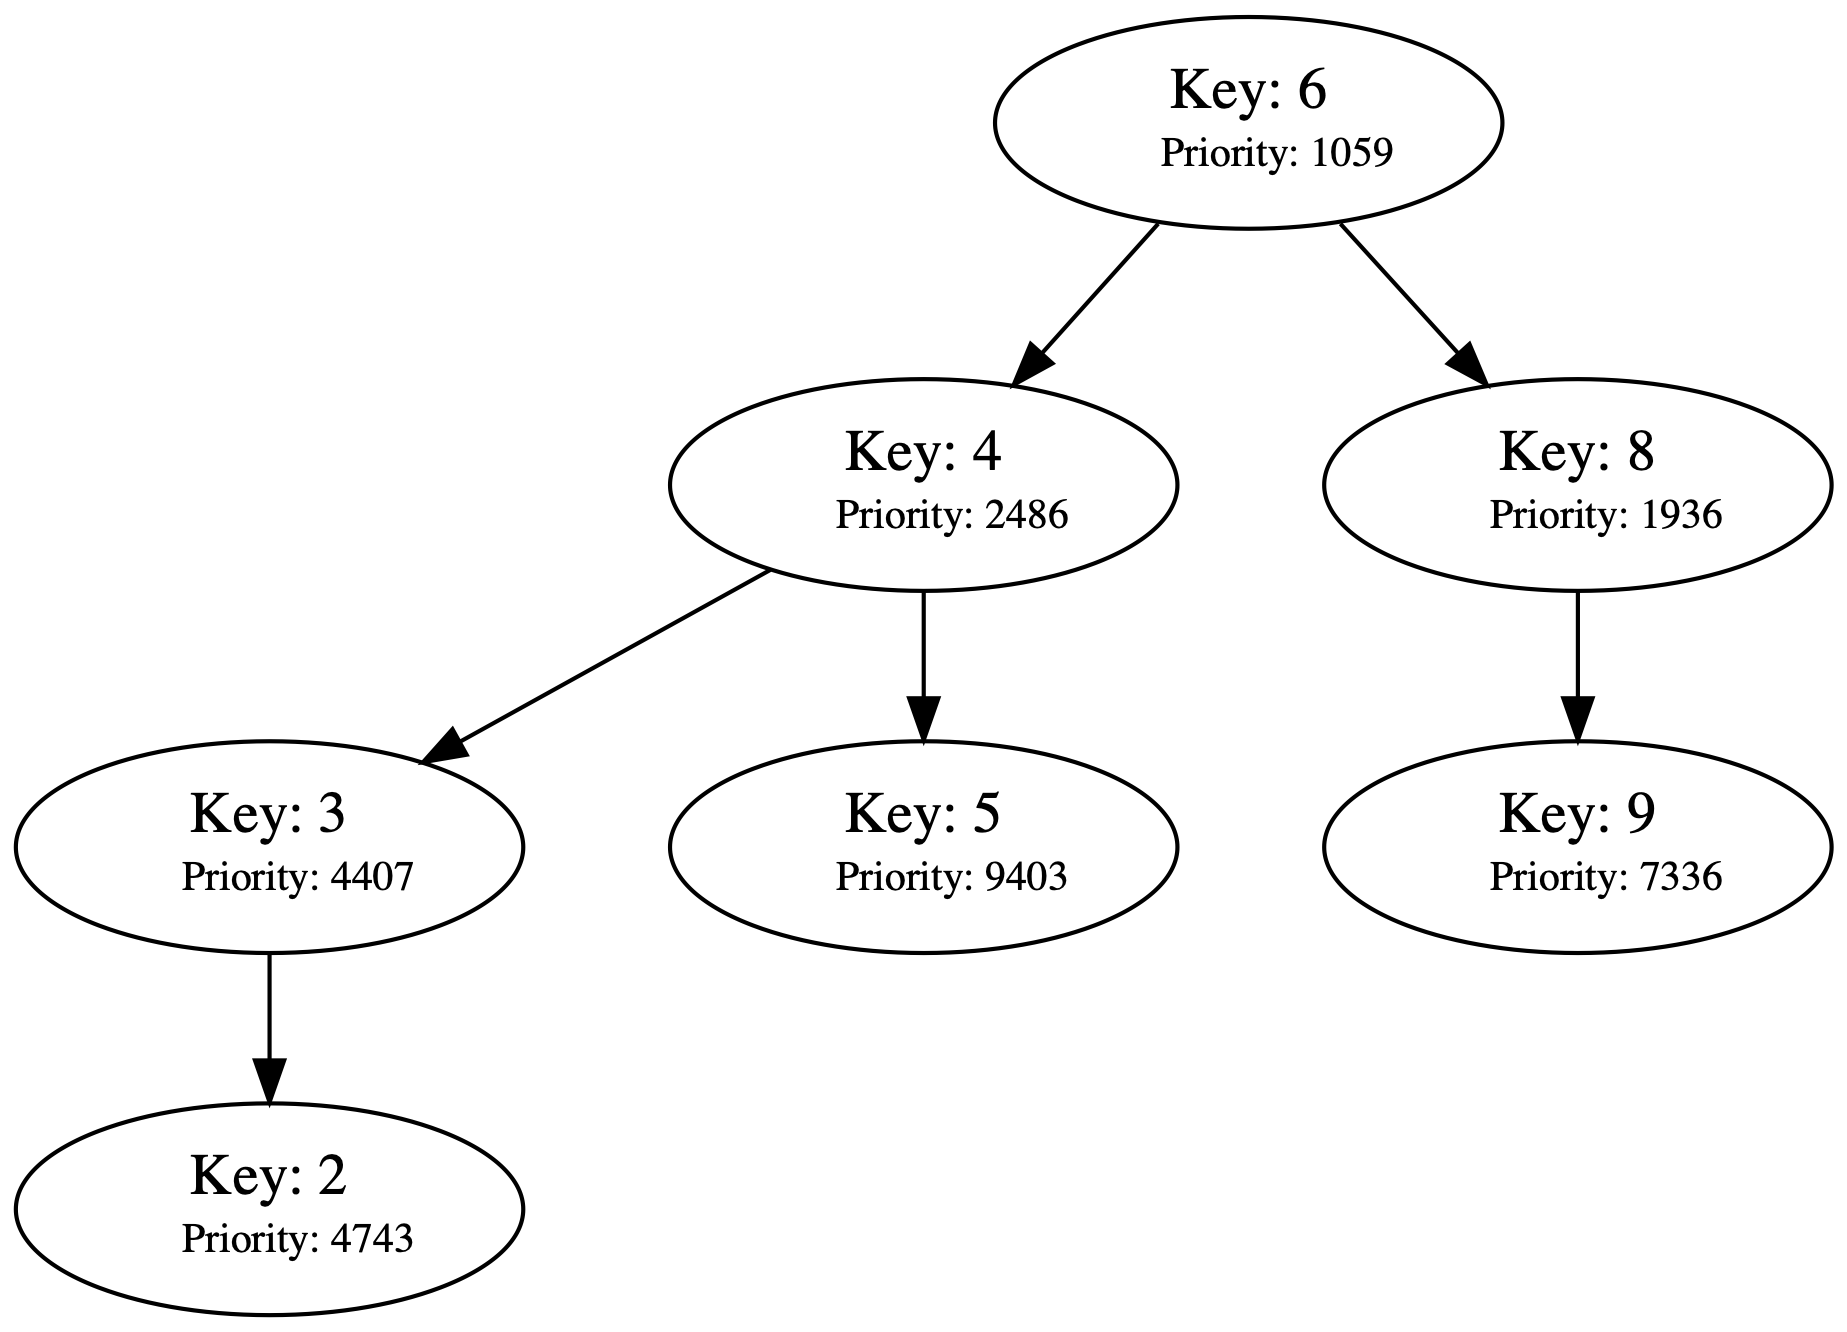
\includegraphics[width=\textwidth]{graphviz/treap.png}
			\caption{Treap}
			\label{fig:Treap}
		\end{figure}
	\subsection{Red Black Tree}
		\subsection{Definición:}
			\par En informática, un Red-Black Tree es una especie de árbol de búsqueda binaria autoequilibrado. Cada nodo del árbol binario tiene un bit extra, y ese bit se interpreta a menudo como el color (rojo o negro) del nodo. Estos bits de color se utilizan para asegurar que el árbol permanezca aproximadamente equilibrado durante las inserciones y eliminaciones.\cite{cormenIntroductionAlgorithms2001}
			
			\par Tienen 5 Propiedades
				\begin{enumerate}
					\item Un nodo es o rojo o negro.
					\item El nodo raíz es negro 
					\item Los nodos hijo de un nodo rojo son negros.
					\item Si un nodo es rojo, entonces sus hijos son negros.
					\item Todos los caminos de un nodo a sus descendientes \texttt{NIL} contienen la misma cantidad de nodos negros.
				\end{enumerate}
		\subsection{Casos de uso:}
		\begin{enumerate}
			\item \textbf{Time-sensitive applications}
			\item \textbf{Geometría computacional}
			\item \textbf{Completely Fair Scheduler}: Maneja la asignación de recursos de la CPU para la ejecución de procesos, y tiene como objetivo maximizar la utilización general del CPU al mismo tiempo que maximiza el rendimiento interactivo. 
		\end{enumerate}
		\subsection{Implementación}
			\subsubsection{Insertar:}
				\begin{enumerate}
					\item Insertar un nodo $z$ rojo.
					\item Se les da un nuevo color a los nodos y se rotan para arreglar las violaciones a las reglas del árbol.
				\end{enumerate}
				\par \textbf{Caso 0: Si $z$ es raíz:}
					\begin{enumerate}
						\item Se le cambia el color a $z$ a negro.
					\end{enumerate}
				
				\par \textbf{Caso 1: Si el tío de $z$ es rojo:}
					\begin{enumerate}
						\item Se le cambia el color al abuelo, papá y tío. 
					\end{enumerate}
			
				\par \textbf{Caso 2: Si el tío de $z$ es negro en forma un triángulo:}
					\begin{enumerate}
						\item Se rota $z$ con su nodo padre.
					\end{enumerate}
				
				\par \textbf{Caso 3: Si el tío de $z$ es negro en línea recta:}
					\begin{enumerate}
						\item Se rota $z$ con su nodo padre. 
						\item Se les cambia de color al abuelo y al padre de $z$.
					\end{enumerate}
	\subsection{Ejemplo en graphviz:}
		\begin{figure}[H]
			\centering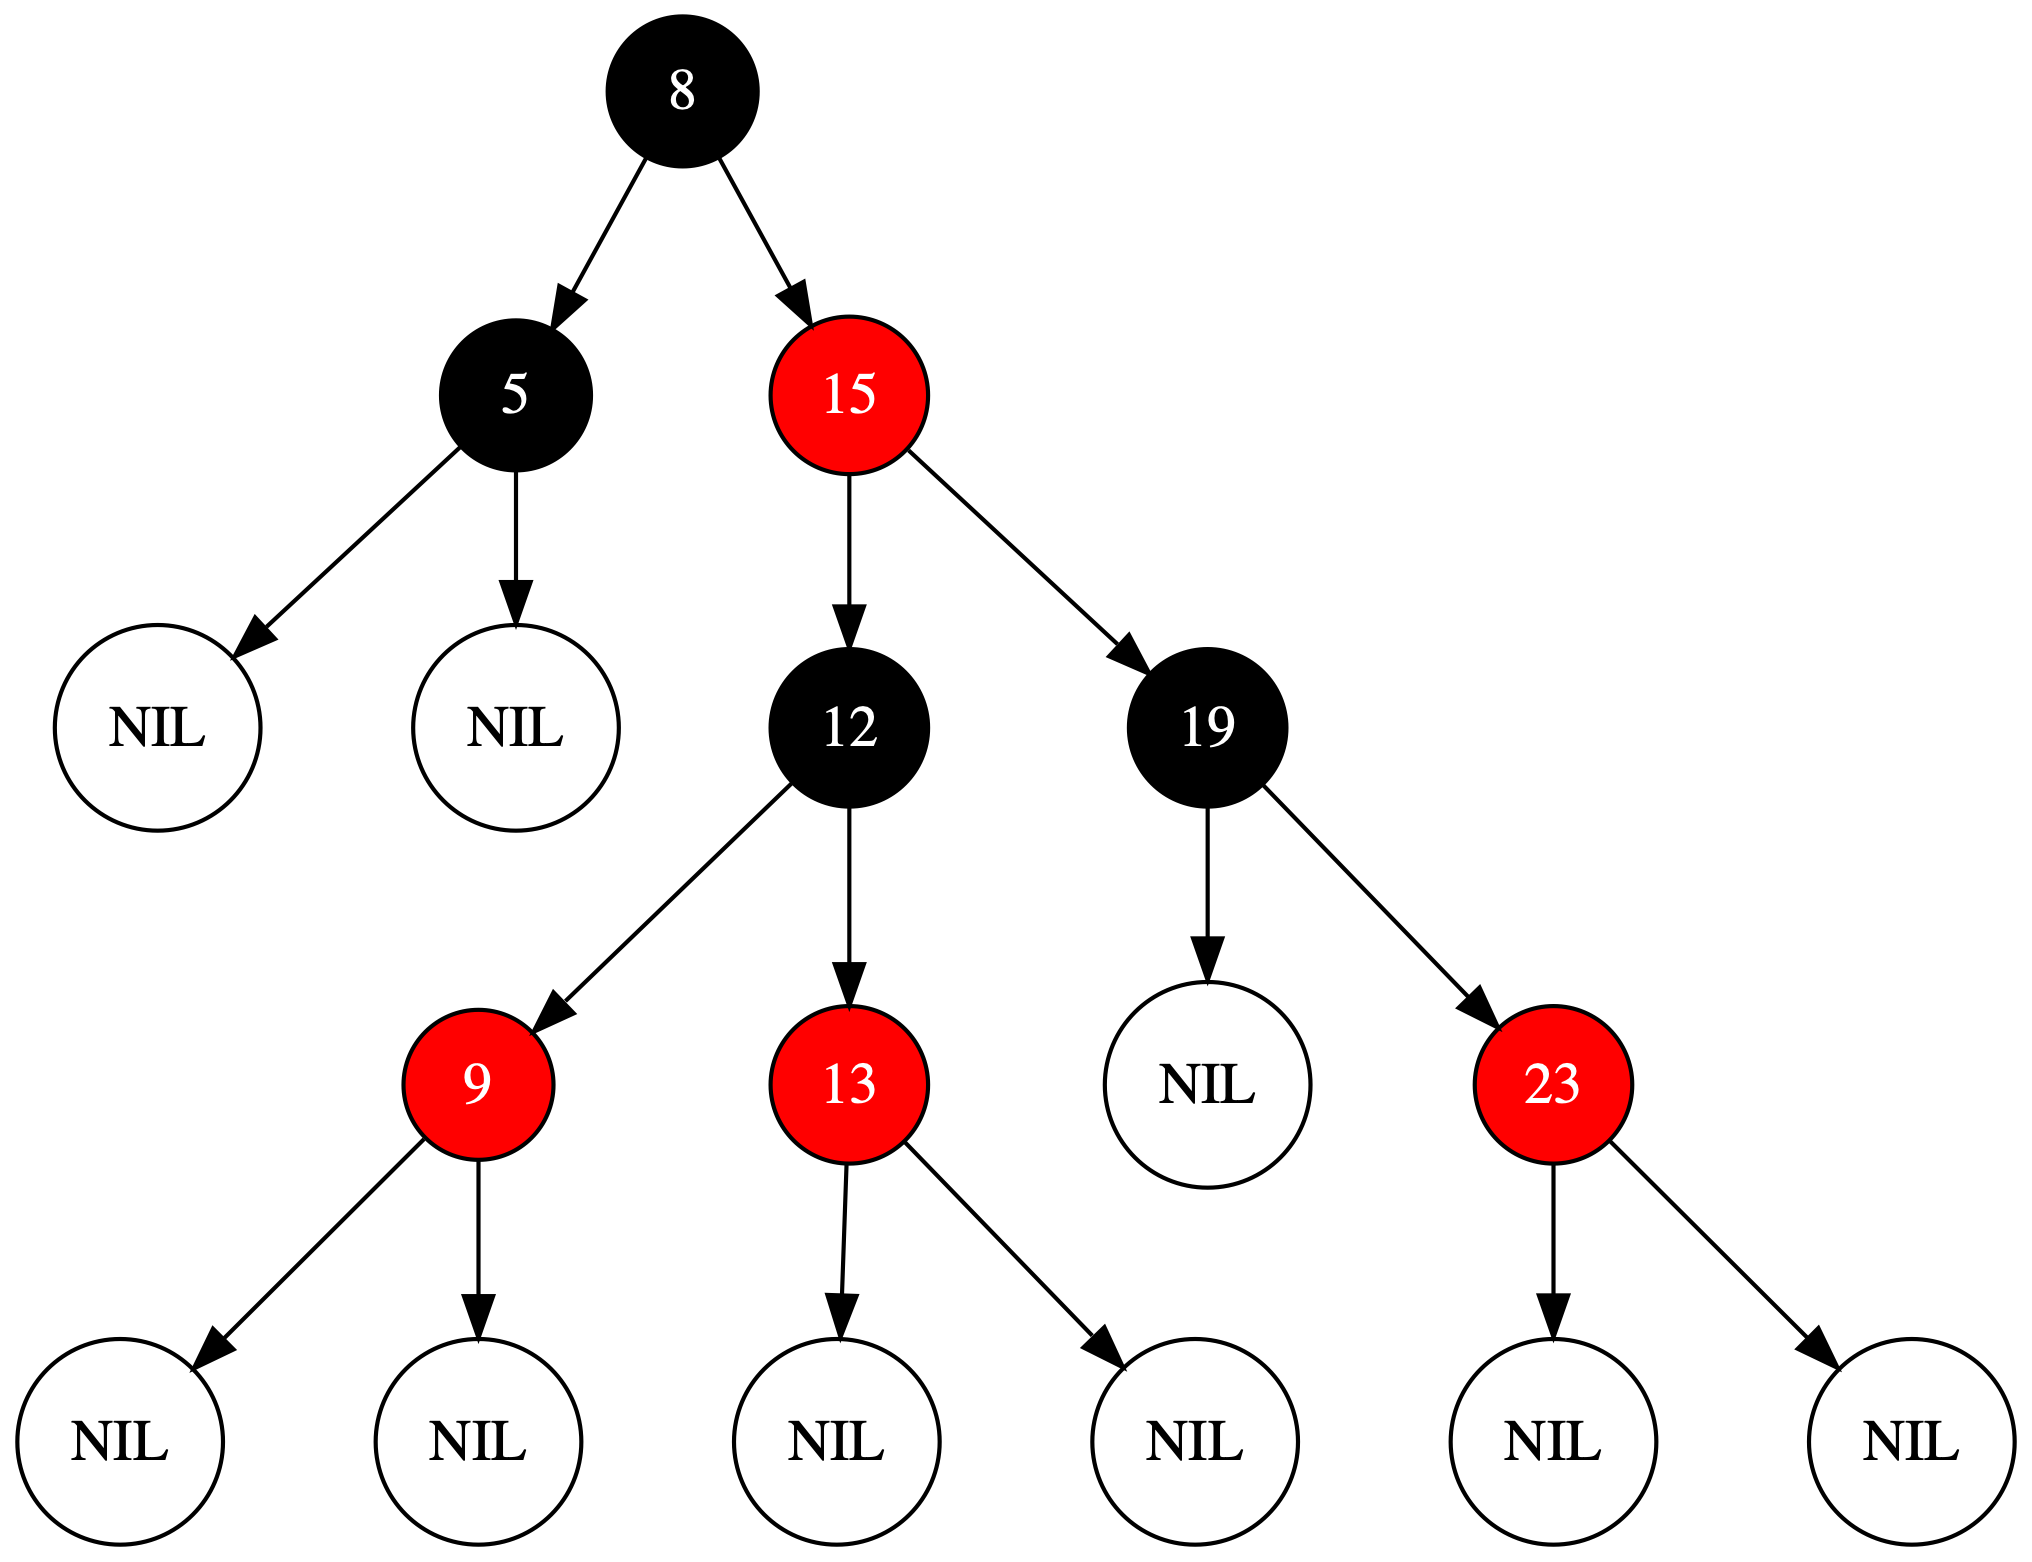
\includegraphics[width=\textwidth]{graphviz/redBlackTree.png}
			\caption{Red Black Tree}
			\label{fig:Red Black Tree}
		\end{figure}
	
\section{HTree \textit{(hashed B-Tree)}}
	\subsection{Definición:}
		\par Un HTree es una estructura de datos de árbol especializada para la indexación de directorios, similar a un árbol B. El algoritmo HTree se distingue de los métodos estándar del árbol B por su tratamiento de colisiones de hash, que pueden causar un \textit{overflow} a través de múltiples hojas y bloques de índice. Los índices HT se utilizan en los sistemas de archivos ext3 y ext4 de Linux, y se incorporaron al núcleo de Linux alrededor de 2.5.40 \cite{tytsoAddExt3Indexed2002}.
		
		\par Contiene dos tipos de bloques en un directorio indexeado.
			\begin{enumerate}
				\item \textbf{DX-block} \textit{(directory indices block)}: Guarda el \texttt{hash-value}/\texttt{block-ID}.
				\begin{enumerate}
					\item \textbf{Hash Value}: El valor en hash de un \textit{entry name}.
					\item \textbf{Block-ID}: Ya sea el número de block lógico de el block hijo, o el siguiente nivel de índice.
				\end{enumerate}
			\item \textbf{DE-block} \textit{(directory entries block)}: Guarda los nombres de los directorios (nombres de archivos).
			\end{enumerate}
	\subsection{Casos de uso:}
		\begin{enumerate}
			\item Directorios grandes en los \textit{filesystems} \texttt{ext3} y \texttt{ext4}.
		\end{enumerate}
	\subsection{Implementación:}
	\subsubsection{Operaciones:}
		\begin{enumerate}
			\item \textbf{Búsqueda}: Busca una entrada de nombre en htree, o busca la entrada de nombre en la ruta htree.
			
			\item \textbf{Insertar entrada de nombre}: Insertar una entrada de nombre en el DE-block en la ruta del árbol.
			
			\item \textbf{Borrar entrada de nombre}: Eliminar una entrada de nombre del DE-block en la ruta htree.
			
			\item \textbf{Dividir DE-block}: Si se inserta una entrada en un DE-block completo, se asigna un nuevo bloque y la mitad de las entradas de nombre del DE-block original se mueven al nuevo bloque.
			
			\item \textbf{Dividir DX-block}: Cuando se asigna un nuevo DE-block, debe insertarse en el DX-block principal. Al insertar un DE-block en un DX-block completo, el DX-block se divide.
		
			\item \textbf{Hacer crecer el árbol}: Un árbol crece si se produce una división de DE-block y todos los DX-block de la trayectoria del árbol están llenos. En este caso se añade otra capa al árbol.
		\end{enumerate}
	\subsubsection{Hash collision:}
		\par Las entradas en el directorio htree son indexadas por un valor hash del nombre. Existe una posibilidad improbable, pero finita, de que dos nombres cualesquiera no generen un valor de hash único. Esto se llama colisión de hash. Si estos nombres se extienden por más de un bloque, entonces la búsqueda de cualquiera de estos nombres necesita iterar en todos estos bloques, y esto debe ser manejado correctamente para PDO.
	\subsection{Ejemplo en graphviz:}
		\begin{figure}[H]
			\centering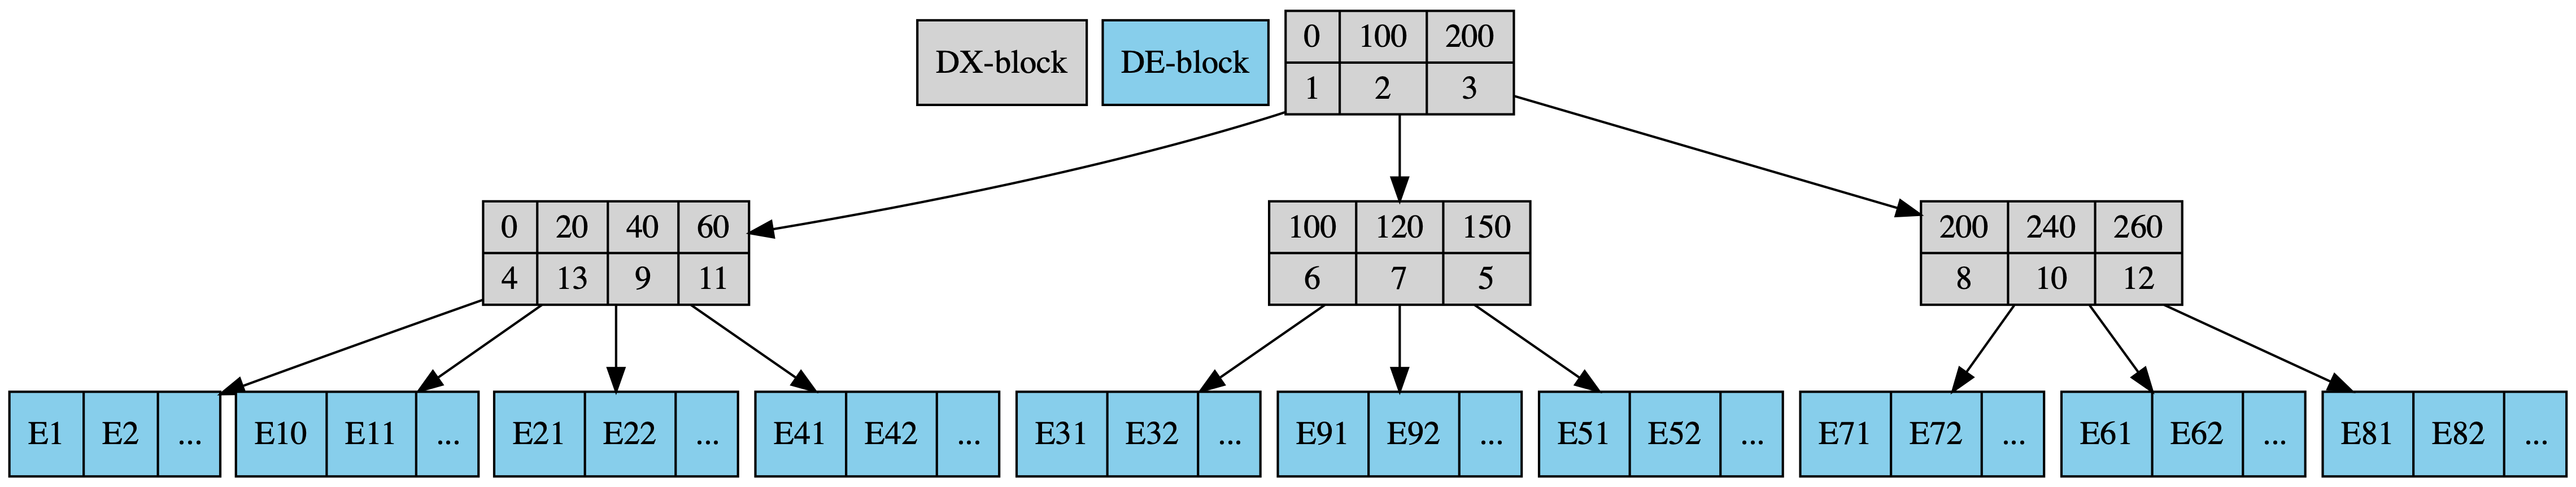
\includegraphics[width=\textwidth]{graphviz/htree.png}
			\caption{Htree}
			\label{fig:Htree}
		\end{figure}
	

		
\newpage
\printbibliography
\end{document}
